% Options for packages loaded elsewhere
\PassOptionsToPackage{unicode}{hyperref}
\PassOptionsToPackage{hyphens}{url}
%
\documentclass[
]{article}
\usepackage{amsmath,amssymb}
\usepackage{lmodern}
\usepackage{iftex}
\ifPDFTeX
  \usepackage[T1]{fontenc}
  \usepackage[utf8]{inputenc}
  \usepackage{textcomp} % provide euro and other symbols
\else % if luatex or xetex
  \usepackage{unicode-math}
  \defaultfontfeatures{Scale=MatchLowercase}
  \defaultfontfeatures[\rmfamily]{Ligatures=TeX,Scale=1}
\fi
% Use upquote if available, for straight quotes in verbatim environments
\IfFileExists{upquote.sty}{\usepackage{upquote}}{}
\IfFileExists{microtype.sty}{% use microtype if available
  \usepackage[]{microtype}
  \UseMicrotypeSet[protrusion]{basicmath} % disable protrusion for tt fonts
}{}
\makeatletter
\@ifundefined{KOMAClassName}{% if non-KOMA class
  \IfFileExists{parskip.sty}{%
    \usepackage{parskip}
  }{% else
    \setlength{\parindent}{0pt}
    \setlength{\parskip}{6pt plus 2pt minus 1pt}}
}{% if KOMA class
  \KOMAoptions{parskip=half}}
\makeatother
\usepackage{xcolor}
\usepackage[margin=1in]{geometry}
\usepackage{graphicx}
\makeatletter
\def\maxwidth{\ifdim\Gin@nat@width>\linewidth\linewidth\else\Gin@nat@width\fi}
\def\maxheight{\ifdim\Gin@nat@height>\textheight\textheight\else\Gin@nat@height\fi}
\makeatother
% Scale images if necessary, so that they will not overflow the page
% margins by default, and it is still possible to overwrite the defaults
% using explicit options in \includegraphics[width, height, ...]{}
\setkeys{Gin}{width=\maxwidth,height=\maxheight,keepaspectratio}
% Set default figure placement to htbp
\makeatletter
\def\fps@figure{htbp}
\makeatother
\setlength{\emergencystretch}{3em} % prevent overfull lines
\providecommand{\tightlist}{%
  \setlength{\itemsep}{0pt}\setlength{\parskip}{0pt}}
\setcounter{secnumdepth}{-\maxdimen} % remove section numbering
\usepackage{booktabs}
\usepackage{wrapfig}
\usepackage{graphicx}
\usepackage{subcaption}
\usepackage[font=footnotesize]{caption}
\usepackage{titling}
\captionsetup[figure]{font=small}
\ifLuaTeX
  \usepackage{selnolig}  % disable illegal ligatures
\fi
\IfFileExists{bookmark.sty}{\usepackage{bookmark}}{\usepackage{hyperref}}
\IfFileExists{xurl.sty}{\usepackage{xurl}}{} % add URL line breaks if available
\urlstyle{same} % disable monospaced font for URLs
\hypersetup{
  hidelinks,
  pdfcreator={LaTeX via pandoc}}

\author{}
\date{\vspace{-2.5em}}

\begin{document}

\hypertarget{iisd-ela-analytical-service-lab-summary}{%
\section{2023 IISD-ELA Analytical Service Lab
Summary}\label{iisd-ela-analytical-service-lab-summary}}

Sonya Havens\\
2024-02-28

\hypertarget{students}{%
\subsection{Students}\label{students}}

\begin{itemize}
\item
  \emph{Jenny Thoroski} - returning for third year in the Analytical
  Service Lab. Worked May to November 24, 2023 in Pod 3 analysing pH on
  the pH meter, conductivity, gran alkalinity, and turbidity on the
  MT-100, and absorbance scans, soluble reactive silica and particulate
  phosphorus on the UV-1800 spectrophotometer. Jenny also conducted an
  instrument cross comparison study, wherein samples were analysed on
  the old Accumet pH meter and the new Orion Star pH meter.
\item
  \emph{Emily Loewen} - New student. Worked from May to the end of
  August, 2023 in Pod 1 Monday through Wednesday conducting sample
  preparation and filtration, then helped with Pod 3 every Thursday and
  Friday analysing particulate phosphorus on the UV-1800
  spectrophotometer and chlorophyll-a on the Trilogy fluorometer.
\item
  \emph{Collette Leclerc} - New student. Worked from September to
  November 24, 2023 in Pod 1 Monday through Wednesday conducting sample
  preparation and filtration, then helped with Pod 3 every Thursday and
  Friday analysing particulate phosphorus on the UV-1800
  spectrophotometer and chlorophyll-a on the Trilogy fluorometer.
\end{itemize}

\hypertarget{instrument-installationimplementation}{%
\subsection{Instrument
installation/implementation}\label{instrument-installationimplementation}}

\underline{Orion Star A211 pH meter}

The Thermofisher Scientific Orion Star A211 pH meter was purchased
April, 2023. Samples were analysed on both the old Fisher Accumet pH
meter and the new Orion pH meter from May to August, 2023. The
comparison report will be completed by May 2024.

\underline{Shimadzu HIC-ESP}

The Shimadzu HIC-ESP, which was purchased in December 2022 and installed
in April 2023, is used for the anlaysis of anaions chloride and sulfate.
Samples collected in 2022 were analysed on the Shimadzu HIC-ESP and were
compared to results from the analysis of these samples at the University
of Alberta Biogeochemical Analytical Service Laboratory (UA-BASL) on a
Dionex Ion Chromatograph. The comparison report
(2023\_ShimadzuIC\_comparison) is complete and can be found in the
IISD-ELA github and all of the 2023 anions samples have been analysed.

\underline{Agilent Microwave Plasma Atomic Emission Spectrometer}

The Agilent Microwave Plasma Atomic Emission Spectrometer (MPAES), which
was purchased in December 2022 and installed July 2023, is used to
measure cations (Ca, Fe, K, Mg, Mn, Mo, Na, and Zn) and particulate
iron.

Particulate iron samples collected from 2019 to 2022 were analysed on
the MPAES and compared with results from the analysis of these samples
measured at the University of Winnipeg on a PerkinElmer AAnalyst 400
Atomic Absorption Spectrophotometer. The comparison report
(2023\_PartFe\_UW\_MPAES\_comparison) is complete and can be found on
the IISD-ELA github.

Cation samples collected in 2022 were analysed on the MPAES and compared
with results from the analysis of these samples measured at the UA-BASL
using a Thermo ICAP-6300 Inductively Coupled Plasma Optical Emission
Spectroscopy. The comparison report will be complete by May 2024. Cation
samples collected in 2023 will be measured on the MPAES following
experiments to determine if an internal standard and/or acid addition is
required to enhance the accuracy and precision of cation measurements.

\pagebreak

\underline{Elementar enviroTOC}

The Elementar enviroTOC, which was purchased in December 2022 and
installed October 2023, is used to measure dissolved organic carbon.
Dissolved organic carbon samples collected in 2022 will be analysed on
the enviroTOC and compared with results from the analysis of these
samples measured at the Fisheries and Oceans Canada Fresh Water
Institute using a Shimadzu TOC-VCPH by May 2024. Dissolved organic
carbon samples collected in 2023 will be measured as soon as the cross
comparison is complete.

\underline{Elementar UNICUBE}

The Elementar UNICUBE, which was purchased in December 2022 and
installed October 2023, is used to measure particulate carbon and
nitrogen. Particulate carbon and nitrogen samples were collected in
duplicate in 2023 with one set sent to the UA-BASL for analysis using
the Exeter CE 440 Elemental Analyzer and one set retained for analysis
on the UNICUBE. The UNICUBE is currently being optimized to improve
accuracy and precision at low concentrations and achieve the lowest
limit of detection possible. Particulate carbon and nitrogen samples
collected in 2023 will be analysed on the UNICUBE following optimization
and cross comparison.

\hypertarget{samples-processed-by-the-iisd-analytical-service-lab}{%
\subsection{Samples processed by the IISD Analytical Service
Lab}\label{samples-processed-by-the-iisd-analytical-service-lab}}

The total number of samples processed by the IISD-ELA Analytical Service
Lab (IISD-ASL) in 2023 was 1162. The following plot displays how many
samples were analysed for each test in 2023.

\begin{figure}[h]
  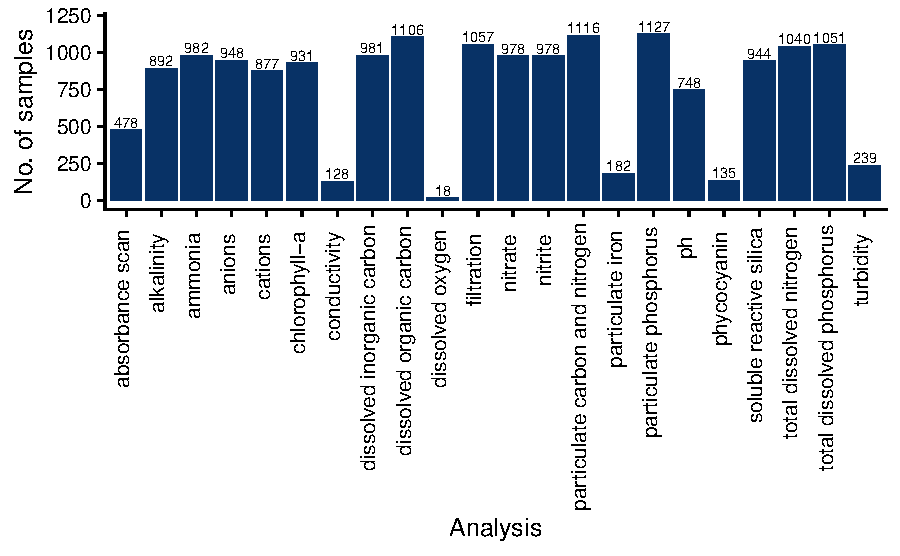
\includegraphics[width=0.85\textwidth]{test_summary_plot.pdf}
  \caption{Number of samples processed for each analysis}
\end{figure}

\hypertarget{proficiency-testing}{%
\subsection{Proficiency testing}\label{proficiency-testing}}

We received a proficiency testing score of ``Good''. The nitrite +
nitrate results from several Rain \& Soft Waters (RN) samples were
biased high and the dissolved inorganic carbon (DIC) results of several
Major Ions in Natural Waters (MI) samples were also biased high.
\pagebreak

The high bias in the nitrite + nitrate RN samples (and one low bias
result) is concerning. While all of the high biased samples required
dilution to fall within the analytical calibration range, dilutions are
a common practice for this analysis and the nitrite + nitrate
concentrations in these samples are representative of typical IISD-ASL
samples. We will need to investigate the cause of this lack of accuracy
and precision in nitrite and nitrate concentrations.

With the exception of one alkalinity sample that was biased low, all of
the other analytical results of RN samples were within acceptable
limits.

\begin{figure}[h]
\centering
  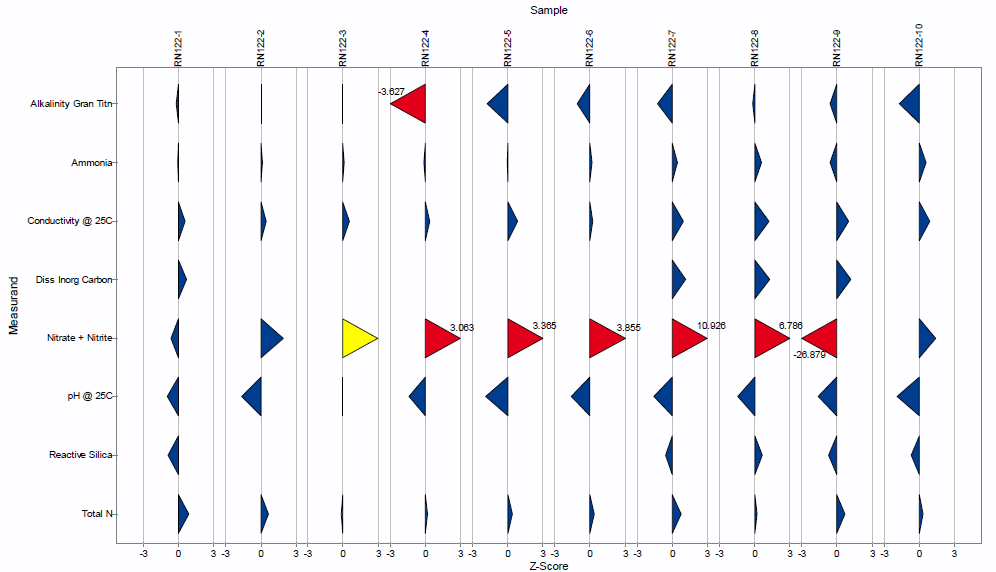
\includegraphics[width=0.8\textwidth]{2023_PT_RN_zscores.png}
  \caption{Z scores for results of rain and soft waters proficiency testing samples}
\end{figure}

The DIC concentrations in the MI samples were substantially higher than
samples collected at the IISD-ELA and thus are not representative of the
appropriate DIC concentration range pertinent for use in the IISD-ASL.
Regardless, the high bias in DIC concentrations of MI samples was due to
the necessity of a very low sample injection volume (0.03-0.05 mL
compared to the typical sample injection volume of 0.25 mL), which
induces a loss of accuracy and precision.

\begin{figure}[h]
\centering
  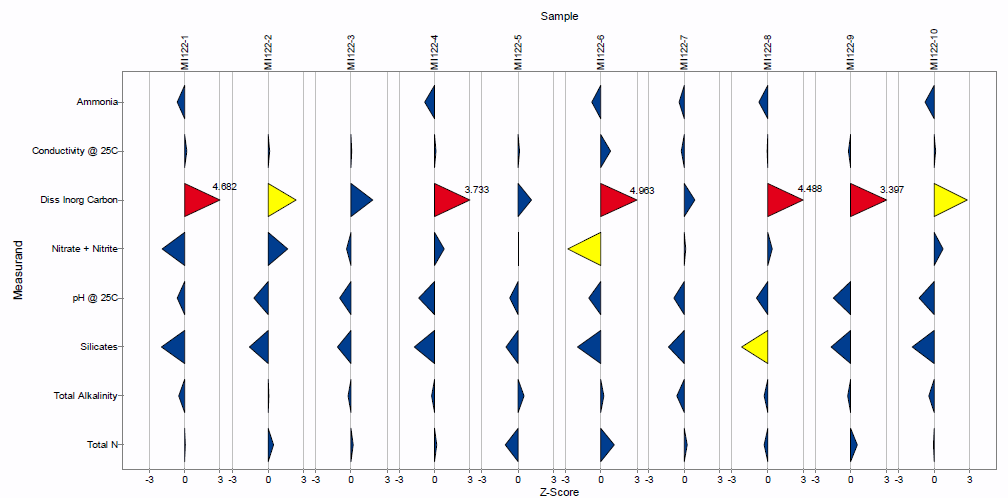
\includegraphics[width=0.8\textwidth]{2023_PT_MI_zscores.png}
  \caption{Z scores for results of major ions and nutrients proficiency testing samples}
\end{figure}
\pagebreak

In addition to the DIC bias described above, one nitrite + nitrate
result and one silicate result were biased low in MI samples. All of the
other analytical results of MI samples were within acceptable limits.

All of the total phosphorus results of the proficiency samples were
within acceptable limits.

\begin{figure}[h]
\centering
  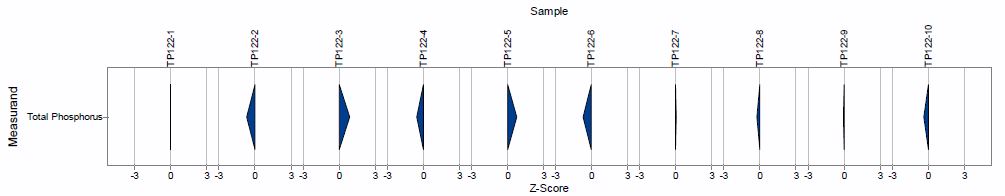
\includegraphics[width=0.99\textwidth]{2023_PT_TP_zscores.png}
  \caption{Z scores for results of total phosphorus proficiency testing samples}
\end{figure}

Two out of ten proficiency testing samples had low biased turbidity
results. These two turbidity results were substantially higher than
turbidity concentrations in samples collected at the IISD-ELA and thus
are not representative of the appropriate turbidity concentration range
pertinent for use in the IISD-ASL.

\begin{figure}[h]
\centering
  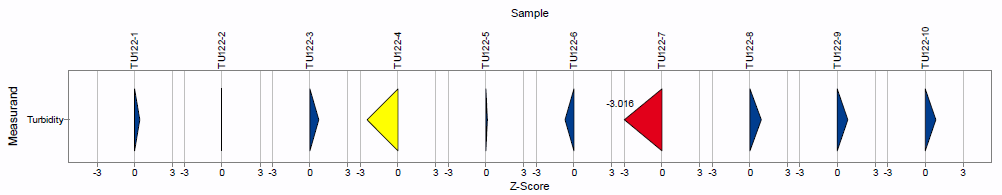
\includegraphics[width=0.99\textwidth]{2023_PT_TU_zscores.png}
  \caption{Z scores for results of turbidity proficiency testing samples}
\end{figure}
\pagebreak

\hypertarget{budget}{%
\subsection{Budget}\label{budget}}

The following plot provides the category breakdown of the 2023-24 fiscal
year (FY) budget forecast and actual expenditures as of 2024-02-28. We
are awaiting the invoice for our laboratory testing expenditures. The
\$25,000 forecast value for the licenses and permits was likely a
decimal place error, as these costs are closer to \$2,500.

\begin{figure}[h]
\centering
  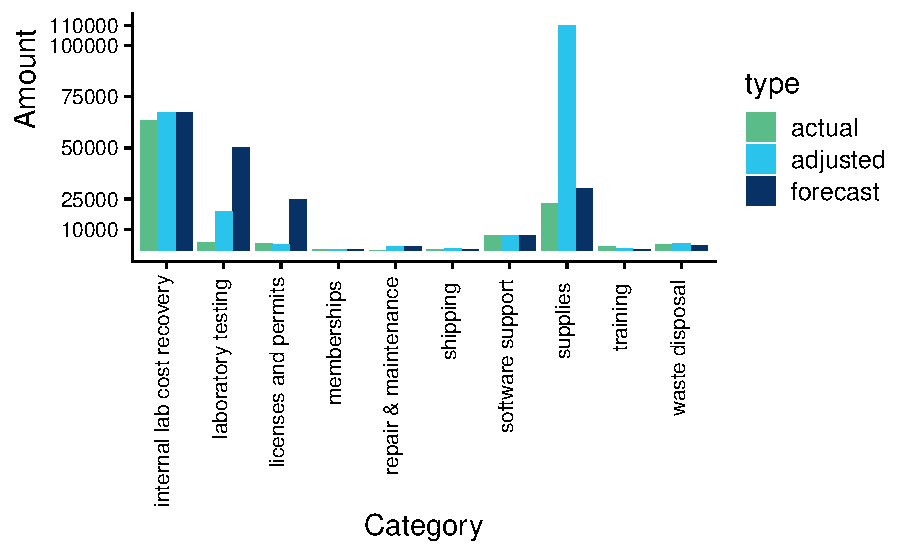
\includegraphics[width=0.99\textwidth]{2023_24FY_budget.pdf}
  \caption{2023-24 fiscal year budget. The internal lab cost recovery represents receivable funds. All other categories are expenditures.}
\end{figure}

The 2023-24 FY budget was adjusted for the September 1, 2023 to March
31, 2024 quarter to procure non-perishable consumables and capital
assets in the 2023-24 FY to reduce costs in the 2024-25, 2025-26, and
2026-27 FY's to accommodate increased costs in these FY's associated
with the build of the Centre for Lake Learning and Climate Change.
Figure 6 provides the category breakdown of the 2023-24 FY budget that
accounts for these adjustments. We were able to bring down laboratory
testing costs down to \textasciitilde\$19,000 from
\textasciitilde\$50,000 by analysing samples from 2022 for the anions,
cations, and dissolved organic carbon method cross comparison
experiments. The supply budget increased from \$30,000 to \$110,000 in
order to procure three years worth of non-perishable supplies in the
2023-24 FY to reduce costs in the 2024-25, 2025-26, and 2026-27 FY's.

\pagebreak

The following plot provides the category breakdown of the 2024-25 FY
budget forecast. The software support forecast will need to be adjusted
to \$11,350 in the 2024-25 FY. I have disputed the software support
costs for our Laboratory Information Management System (Sample Master®)
for several years now to bring the costs down to what I considered
justifiable. The software support cost are supposed to be calculated as
18\% of the software costs at purchase. However, this was based on
software costs before discounts, and they considered only having five
licenses, as opposed to unlimited licenses, a discount (\$17,138.10),
which I disputed as inappropriate. I had also argued to have our beta
testing discount included in the software support cost calculation as I
found it inappropriate to have to pay to communicate with support to
assist them with improving their software. The beta testing portion has
ended, so this adjustment to the software support cost is no longer
available and I have been informed by the Accounts Manager that starting
in 2024 they will no longer be acquiescing to my arguments and the
support costs will increase to approximately \$11,350.

The internal lab cost recovery is likely an underestimate as additional
project analysis requests are often received in April.

\begin{figure}[h]
\centering
  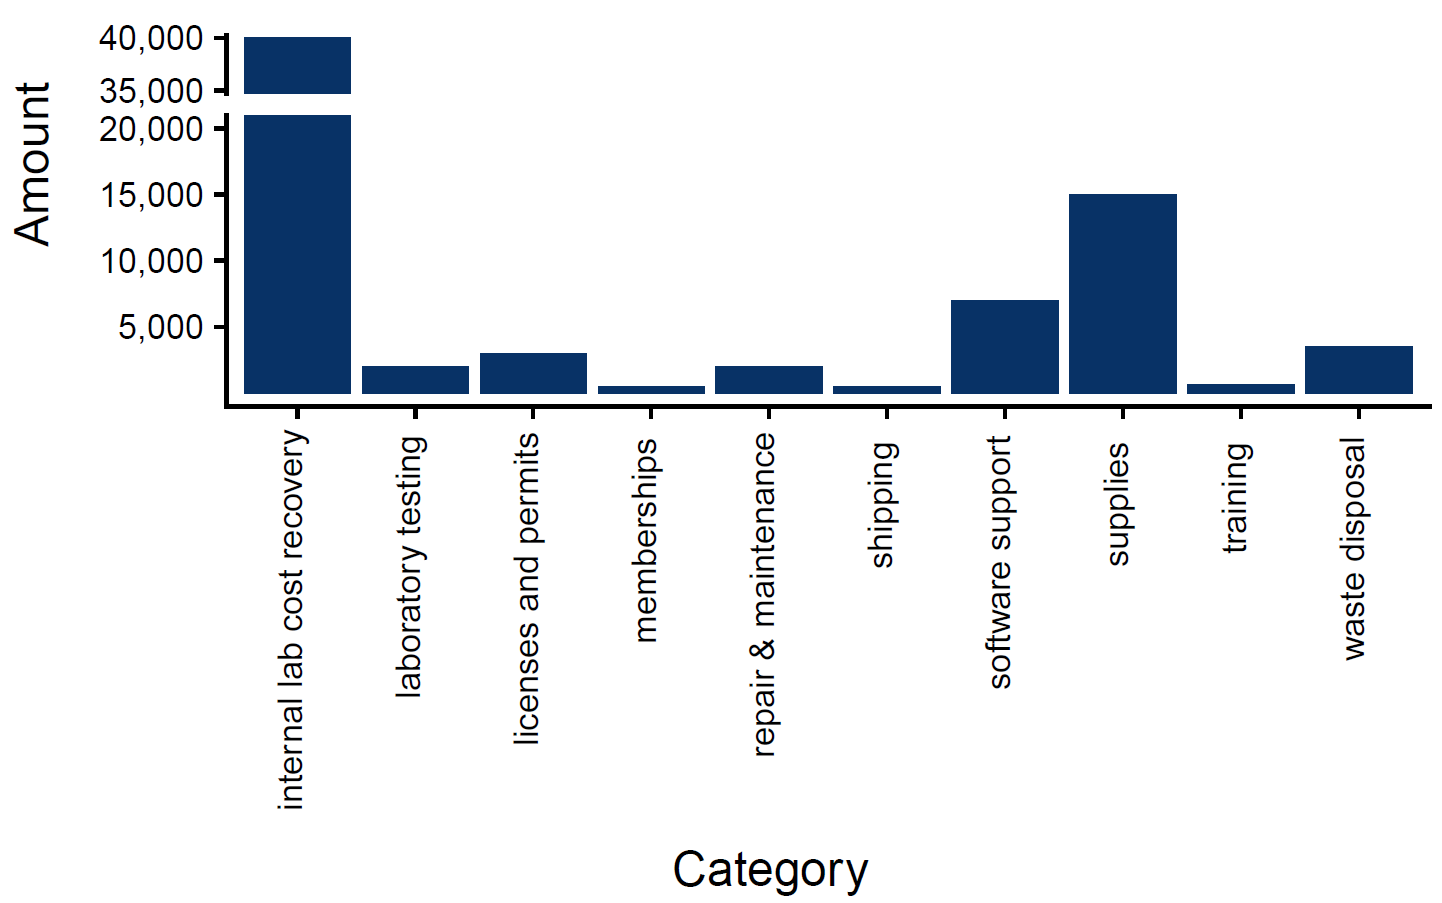
\includegraphics[width=0.99\textwidth]{FY2024_25_budget_snip.png}
  \caption{2024-25 fiscal year budget. The internal lab cost recovery represents receivable funds. All other categories are expenditures.}
\end{figure}
\pagebreak

\hypertarget{capital-asset-investments}{%
\subsection{Capital asset investments}\label{capital-asset-investments}}

The following plot provides the breakdown of the capital assets budget
forecast and actual expenditures in the 2022-23 FY. All of the 2022-23
FY capital assets have been purchased and installed. The actual costs of
the Autoclave and Centrifuge were slightly higher than forecasted. All
other purchases were within the forecasted budget.

\begin{figure}[h]
\centering
  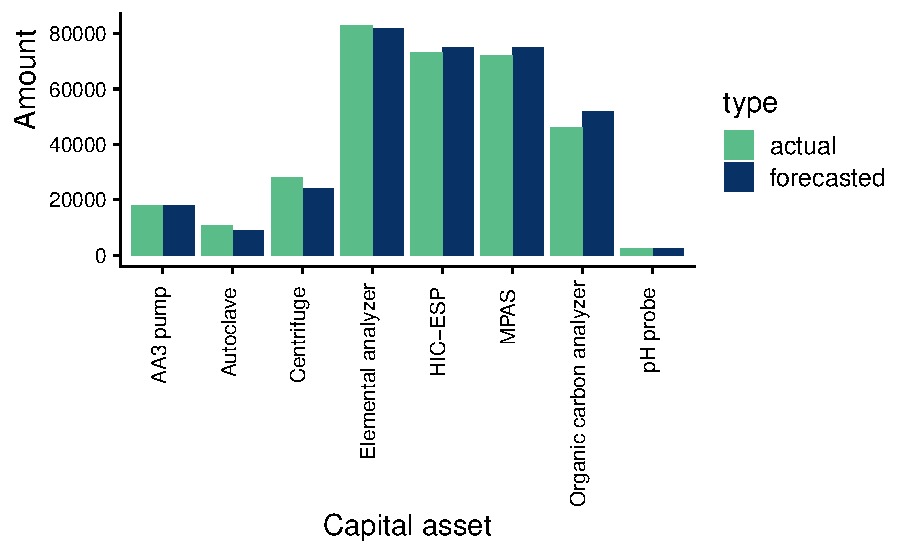
\includegraphics[width=0.99\textwidth]{2022_23FY_capital_assets.pdf}
  \caption{2022-23 capital assets expenditures}
\end{figure}

The following capital assets may be purchased in the final quarter
pending approval. If not purchased this fiscal, they will be procured in
the 2024-25 or 2025-2026 FY's.

\begin{figure}[h]
\centering
  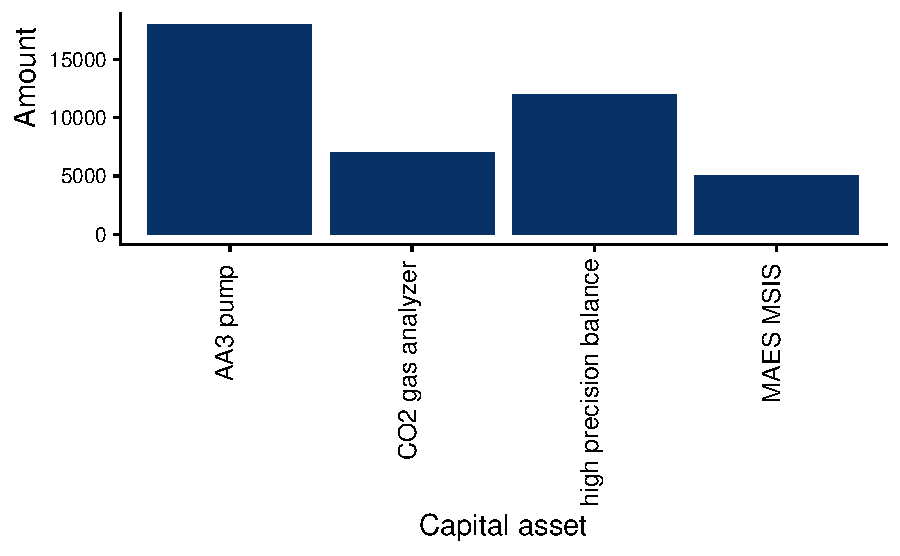
\includegraphics[width=0.6\textwidth]{2023_24FY_capital_assets.pdf}
  \caption{2023-24 capital asset expenditures}
\end{figure}
\pagebreak

\hypertarget{cost-recovery}{%
\subsection{Cost recovery}\label{cost-recovery}}

The following plot breaks down the analytical costs by project. The
Blanks, Broadscale monitoring, Diversion, FAACTS, LTER, and Proficiency
testing, and SHRRIMP project costs are covered by core funding. The 2023
total cost recovery for the externally funded projects was \$70,502.96.

\begin{figure}[h]
\centering
  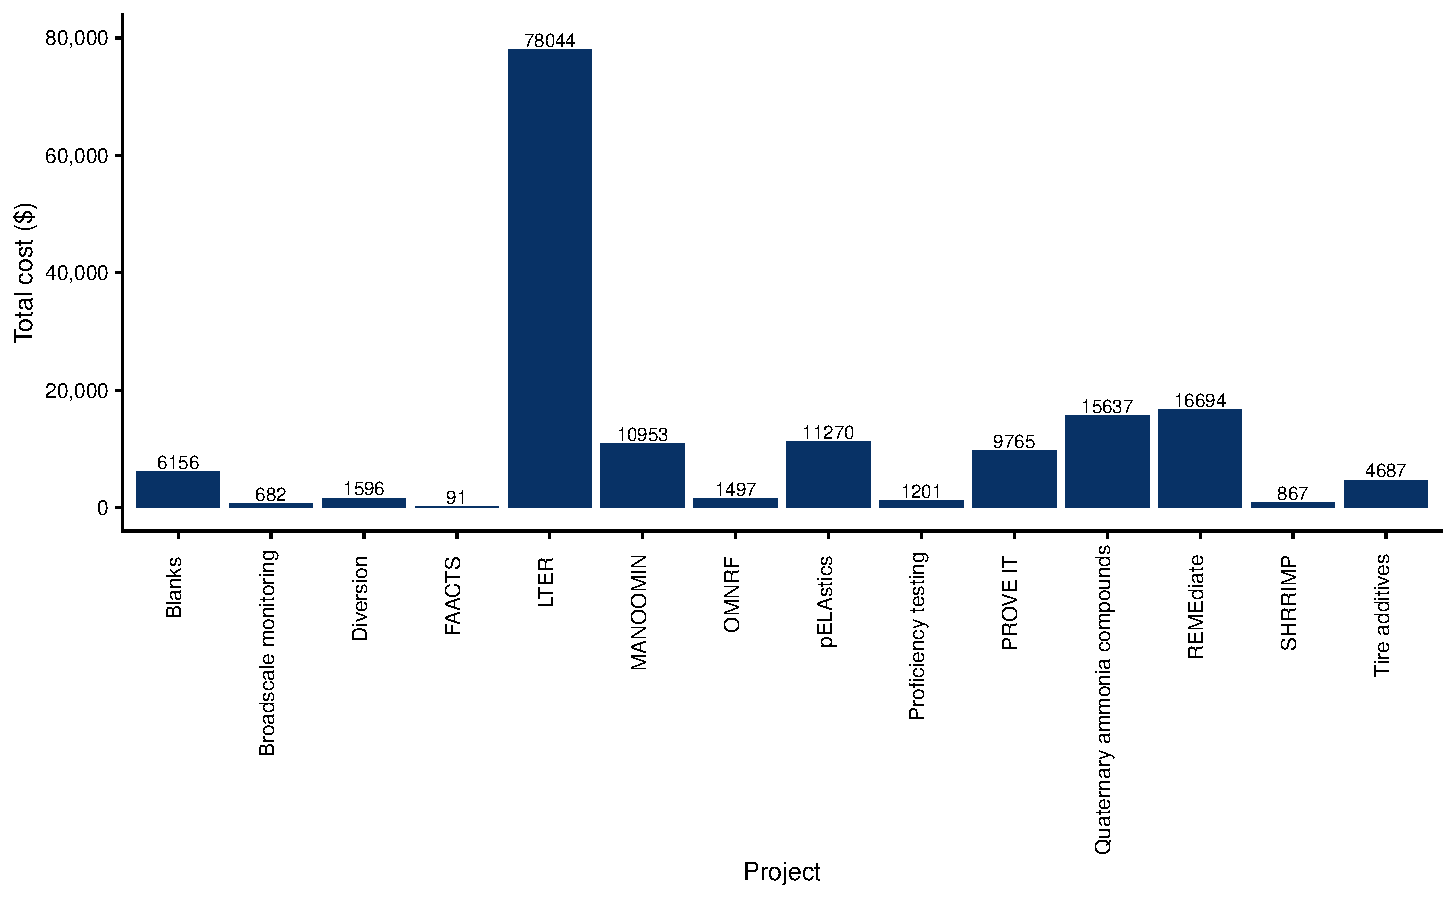
\includegraphics[width=0.99\textwidth]{costs_summary_plot.pdf}
  \caption{Analytical costs for each project}
\end{figure}

\end{document}
